\chapter{Àlgebra Lineal}\label{algebra}
Quan vaig començar a buscar informació sobre computació quàntica, en vaig ràpidament donar compte que necessitava molt més coneixement matemàtic, degut a que no entenia gairebé res dels llibres sobre computació quàntica. Arran aquell temps, una serie de vídeos sobre àlgebra lineal en va captar l’atenció, que es justament la branca de les matemàtiques sobre la qual es basa la computació quàntica. Els vídeos son les lliçons que dona el Professor Gilbert Strang al Institut Tecnològic de Massachusetts (MIT en anglès) \cite{LA_OCW_strang, LA2_OCW_strang}. Una vegada havia vist gairebé tots els vídeos, ja tenia bastants conceptes apresos. 

Aquelles lliçons es van ajudar a entendre les matemàtiques de \textit{Quantum Computation and Quantum Information} \cite{QCandQI} i \textit{Quantum Computing: A Gentle Introduction}. A poc a poc, vaig anar aprenent els fundaments matemàtics de la computació quàntica i mecànica quàntica.

En aquesta secció aniré explicant els conceptes bàsics de l'àlgebra lienal, per formar els coneixements en matemàtiques necessaris per poder comprendre aquest treball. 

\section{Vectors i Espais Vectorials}
Els objectes fonamentals de l'àlgebra lineal són els espais vectorials. Un espai vectorial es el conjunt de tots els vectors que tenen les mateixes dimensions. Per exemple  $\mathbb{R}^{3}$ seria el espai vectorial de tots els vectors de 3 dimensions, aquests vectors normalment s'utilitzen per representar punts en un espai tridimensional. En computació quàntica un tipus d'espais vectorials en concret són utilitzats: Els espais de Hilbert, en altres paraules, un espai vectorial amb un producte interior \cite{QCandQI:GramSchmidt}. Els espais de Hilbert segueixen un conjunt de productes i compleixen unes certes normes, en aquest capítol presentaré una part d'aquestes normes i productes, la quantitat que és necessària. S'ha de tenir en compte que els espais de Hilbert són molt més complicats que el que es representa en aquest treball, també que d'aquí en endavant, quan mencioni espai vectorial hem referiré a un espai de Hilbert, d'ha no ser que s'especifiqui el contrari. 

Els espais vectorial estan definits per les seves bases, un set de vectors $B = \{\ket{v_1}, \dots, \ket{v_n}\}$ es una base vàlida per l'espai $V$, si cada vector $\ket{v}$ en l'espai es pot escriure com $\ket{v} = \sum_i a_i \ket{v_i}$ per $\ket{v_i} \in B$. Els vectors en $B$ són linealment independent entre ells.

La notació estàndard pels conceptes de  àlgebra lienal en mecànica quàntica es la notació de Dirac, en la qual es representa un vector com $ \ket{\psi} $. On $\psi$ es la etiqueta del vector. Un vector $ \ket{\psi} $ amb $n$ dimensions també pot ser representat com una matriu columna que te la forma: 
$$
\ket{\psi} = 
\begin{bmatrix}
	z_{1} \\
	z_{2} \\
	\vdots \\
	z_{n-1} \\
	z_{n}
\end{bmatrix}
$$

On els nombres complexes $(z_{1}, z_{2}, \dots , z_{n-1}, z_{n} )$ són els seus elements. Un vector escrit com a $\ket{\psi}$ també s'anomena \textit{ket}.

La adició d'un par de vectors en un espai de Hilbert es definida per \footnote{Els vectors d'aquesta definició tenen els seus elements representats per la seva etiqueta i un subscrit e.g. el vector $\ket{\psi}$ te un element qualsevol $\psi_{1}$ i el seu primer element es $\psi_{1}$. Aquesta notació es seguirà utilitzant al llarg del treball.}:
$$
\ket{\psi} + \ket{\varphi} = \begin{bmatrix} \psi_{1} \\ \vdots \\ \psi_{n} \end{bmatrix} +
\begin{bmatrix} \varphi_{1} \\ \vdots \\ \varphi_{n} \end{bmatrix}
$$

A més a més, hi ha una multiplicació per un escalar\footnote{Un numero qualsevol en $\mathbb{R}$.} definida per:
$$
  z\ket{\psi} = z\begin{bmatrix} \psi_{1} \\ \vdots \\ \psi_{n} \end{bmatrix} = \begin{bmatrix} z \psi_{1} \\ \vdots \\ z \psi_{n} \end{bmatrix}
$$
On $z$ es un escalar i $\ket{\psi}$ un vector. Cal que notar que cada element del vector es multiplicar per el escalar.

Degut a que els espais de Hilbert son complexos tenen un conjugat complex definit per escalar com a: Per un escalar complex $z=a +bi$, el seu conjugat $z^*$ es igual a $a-bi$. 

Aquesta noció pot ampliar per a vectors i matrius, agafant el conjugat de totes les seves entrades/elements:
$$
\ket{\psi}^{*} = 
	\begin{bmatrix} \psi_{1} \\ \vdots \\ \psi_{n} \end{bmatrix}* = \begin{bmatrix} \psi_{1}^* \\ \vdots \\ \psi_{n}^* \end{bmatrix}
$$
$$
A^{*} = 
	\begin{bmatrix} 
	A_{11} & \cdots & A_{1n}\\ 
	\vdots & \ddots & \vdots \\ 
	A_{m1} & \cdots & A_mn
\end{bmatrix}^* 
= \begin{bmatrix} 
	A_{11}^* & \dots & A_{1n}^*\\ 
	\vdots & \ddots & \vdots \\ 
	A_{m1}^* & \cdots & A_mn^*
\end{bmatrix}
$$
Amb $\ket{\psi}$ sent un vector de dimensions $n$, i $A$ sent una matriu de dimensions $m \times n$.

Un altre concepte important es la transposada, representada per el supercrit $T$ que "rota" un vector o una matriu. Un vector columna amb una dimensió $n,1$ es transforma amb un vector fila amb una dimensió $1,n$\footnote{En realitat els vectors columna son matrius amb dimensió $n,1$ però he estat ometent el 1. Quan hem refereixo a les dimensions de un vector qualsevol, només diré un numero, no obstant, especificaré si és un vector columna o un vector fila.}:
$$
\ket{\psi}^{T} = 
	\begin{bmatrix} \psi_{1} \\ \vdots \\ \psi_{n} \end{bmatrix}^T = \begin{bmatrix} \psi_{1} & \dots & \psi_{n} \end{bmatrix}
$$

El mateix és veritat per les matrius, una matriu $m\times n$ transposada es converteix en una matriu $n \times m$. Per exemple:
$$
A^T = \begin{bmatrix}
	 2 & 3 \\
	 6 & 4 \\
	 2 & 5 
\end{bmatrix}^T = \begin{bmatrix}
 2 & 6 & 2 \\
 3 & 4 & 5
\end{bmatrix}
$$

La combinació de un conjugat complex i la transposada s'anomena el conjugat Hermitià, la seva notació es una $\dagger$ supercrita. Per un vector $\ket{\psi}$ el seu conjugat Hermitià $\ket{\psi}^\dagger$ és:
$$
\ket{\psi}^\dagger = (\ket{\psi}^*)^T =  \begin{bmatrix} \psi_{1}^* & \dots & \psi_{n}^* \end{bmatrix} = \bra{\psi}
$$
El conjugat Hermitià compleix que $\ket{\psi}^\dagger = \bra{\psi}$ i $\bra{\psi}^\dagger = \ket{\psi}$.

El conjugat Hermitià de un vector columna $\ket{\psi}$ s'anomena \textit{bra} o vector dual. En la notació de Dirac un vector dual s'escriu com $\bra{\psi}$.

\section{Operadors Lineals}
Per poder operar amb vectors i fer operacions amb ells, s'utilitzen les matrius, que també son denominades mapes lineal o operadors lineals, que són noms que descriuen millor com funcionen aquests objectes. La definició formal de un operador lineal pot ser bastant complicada, per aquesta raó, utilitzaré termes més informals al en aquesta secció. 

Bàsicament, un operador lineal transforma un vector en un altre vector, aquest vector poden o no ser de espais diferents \cite{LR_done_right:linear_map}. Més formalment, per un vector $\ket{v}$ en un espai $V$ i un vector $\ket{w}$ en un espai $W$, un operador lienal $A$ entre els vectors, fa l'acció:

$$
A \ket{v} = \ket{w}
$$
En altres paraules, l'operador mapa un element del espai vectorial $V$ cap a un espai vectorial $W$.
Els operadors lineals han de complir les següents operacions:
\begin{enumerate}
	\item Adició de Vectors: \\
	Per els vectors $\ket{\psi}$ i $\ket{\varphi}$ en un mateix espai vectorial, i un operador lienal $A$:
	$$ A(\ket{\psi} + \ket{\varphi}) = A\ket{\psi} + A\ket{\varphi}$$ 
	\item Multiplicació Escalar:\\
	Per el vector $\ket{\psi}$, el escalar $z$ i el operador lienal $A$:
	$$ A(z\ket{\psi}) = z A \ket{\psi}$$
\end{enumerate}

Aquestes afirmacions tenen que ser veritat per tots els vectors i tots els escalars en els espais on els operadors actuen. Cal notar que un operador lineal no te perquè ser una matriu necessàriament, fer exemple, les derivades i les integrals son operadors lienals, això es pot provar fàcilment al veure que compleixen els criteris especificats posteriorment. No obstant, les derivades i les integrals usualment no s'apliquen a vectors, sinó a les funcions, però es possible aplicar-les a vectors \footnote{No et preocupis, que es clar que les aplicaré a vectors :D.}.

Les matrius només son la representació matricial del operadors lienals \cite{LR_done_right:matrix}.

	\subsection{Tipus d'Operadors Lineals}
En la secció actual, exposaré els tipus bàsics d'operadors lienals que són indispensables en la teoria presentada en aquest capítol i la rest del treball.

\begin{enumerate}
	\item \textbf{Operador Zero} \\
	Qualsevol espai vectorial té un vector zero expressat en notació de Dirac com a $0$, degut a que $\ket{0}$ es un altre concepte totalment diferent en CQ i IQ\footnote{Computació Quàntica i Informació Quàntica.}. El vector zero es aquell vector que per qualsevol vector $\ket{\psi}$ i qualsevol escalar $z$, es compleix que:	
	$\ket{\psi} + 0 = \ket{\psi} $ i $z0 = 0$. \\
	El operador zero també s'escriu com a $0$ i es defineix com l'operador que mapa qualsevol vector al vector zero: $0\ket{\psi} = 0 $.  
	
	\item \textbf{Matriu inversa} \\
	Un matriu quadrada\footnote{Una matriu quadrada és una matriu amb dimensions $n\times n$, on $n \in \mathbb{N}$.} $A$ és invertible si existeix una matriu $A^{-1}$ de manera que $AA^{-1}=A^{-1}A$. $A^{-1}$ es la matriu inversa de $A$. La manera més ràpida de saber si una matriu es invertible es veient si el seu determinant no és zero.

	\item \textbf{Operador Identitat} \\
	Per a qualsevol espai vectorial $V$ existeix un operador identitat $I$ que es definit com $I\ket{\psi} = \ket{\psi}$, aquest operador no fa cap canvi al vectors als quals opera. Cal notar també que per qualsevol matriu $A$ i la seva inversa és veritat que $AA^{-1} = I$
	
	\item \textbf{Operador Unitari} \\
	Un operador unitari es qualsevol operador que no altera la norma dels vectors al quals es aplicat, per tant, una matriu es unitària si $AA^\dagger = I$
	Per convertir qualsevol operador en unitari, es divideix les seves entrades entre la norma del operador. 
	
	\item \textbf{Operadors Hermitians} \\
	Un operador Hermitià o \textit{self-adjoint operator} en anglès, es qualsevol operador que el seu conjugat Hermitià es ell mateix: $A = A^\dagger$ \\
	Una altre cosa a tenir en compte es que existeix un operador únic $A$ en un espai de Hilbert, de manera que per qualsevol vectors $\ket{\psi}$ i $\ket{\varphi}$, es compleix que:
	$$
	\bra{\psi} (A \ket{\varphi}) = (A^\dagger\bra{\psi})\ket{\varphi}
	$$ 
	Aquest operador es conegut com el \textit{adjoint} o conjugat Hermitià de $A$.
	
\end{enumerate}

\section{Producte Interior i Producte Exterior}

\subsection{Producte Interior}
Un vector dual $\bra{\psi}$ i un vector $\ket{\varphi}$ combinats formen el producte interior $\bra{\psi}\ket{\varphi}$, el qual efectua una operació que agafa els dos vectors com a input i produeix un nombre complex com a output:
$$
\bra{a}\ket{b} = a_1 b_1 + a_2 b_2 + ... + a_{n-1} b_{n-1} + a_n b_n = z
$$
Amb $z, a_i, b_i \in \mathbb{C}$. Quan hem refereixo a un producte interior, normalment diré "el producte interior de dos vectors", quan en realitat es una operació entre un vector dual i un vector.

El equivalent d'aquest producte en un espai real de dos dimensions $\mathbb{R}^2$ es el producte escalar, que es expressat com a :
\begin{equation}
	\bra{a}\ket{b} = \norm{\ket{a}}_2 \cdot \norm{\ket{b}}_2 \cos \theta 
	\label{eq:dot_product}
\end{equation}


Amb $\norm{\cdot}_2$ sent la norma $\ell^2$  definida com a $\norm{\ket{\psi}}_2 = \sqrt{\psi_{1}^2 + \cdots + \psi_{n}^2}$ amb $\theta$ sent l'angle entre els vectors $\ket{a}$ i $\ket{b}$. Com he dit l'equació \eqref{eq:dot_product} és equivalent al producte interior, no obstant, segons el que he vist, no es usada àmpliament ja que interpretar $\theta$ com un angle entre vectors de dimensions altes no té molt de sentit. En contrast, he vist aquest producte presentat en la seva interpretació geomètrica\footnote{Els detalls exactes de l'interpretació geomètrica estan fora del domini d'aquest treball, malgrat que m'agradaria molt parlar sobre el tema.} com el producte entre un vector fila i un vector columna: 
% The Geometry of Linear Equations: https://www.youtube.com/watch?v=ZK3O402wf1c&list=PL3CCC70370BD3FD48&index=1
% The four Fundamental Subspaces: https://www.youtube.com/watch?v=nHlE7EgJFds
$$
\bra{a}\ket{b} = \begin{bmatrix}a_1  \cdots  a_n \end{bmatrix} \begin{bmatrix} b_{1} \\ \vdots \\ b_{n} \end{bmatrix}
$$

Ja he definit la norma $\ell_2$ com l'arrel quadrada de la suma del elements d'un vector al quadrat:
$$
\norm{\ket{a}}_2 = \sqrt{\sum_{i} \abs{a_{i}}^2}
$$
No obstant, la definició més comú es basa en el producte interior. Com es pot veure el producte interior de un vector per ell mateix es la suma de les seves entrades al quadrat:
$$
\bra{a}\ket{a} = a_1 a_1 + \cdots + a_n a_n = a_1^2 + \cdots +  a_n^2 \\= \sum_{i} \abs{a_i}^2
$$
Per tant, la norma pot ser definida com l'arrel quadrada del producte interior d'un vector:
\begin{equation}
\norm{\ket{a}}_2 = \sqrt{\bra{a}\ket{a}}
\label{eq:norm}
\end{equation}
Quan la norma es aplicada a un vector bidimensional, es pot veure que es lo mateix que la longitud Euclidiana d'aquell vector, això es perquè realment son el mateixos conceptes, tot i això, la norma es el concepte de longitud però generalitzat a vectors de dimensions altes. 

Pel el que jo entenc algunes propietats de la longitud d'un vector bidimensional no es mantenen amb la norma d'un vector que te més de 2 dimensions. En altres paraules, la norma es comporta en certes maneres com la distancia des de d'origen (que es la definició de la longitud), per tant, no són exactament lo mateix. A més d’això, hi han diferents tipus de normes que s'utilitzen en diversos escenaris. Aquesta es la raó per la qual en refereixo a la norma, com la norma $\ell^2$. A aquesta norma també se li diu norma Euclidiana \cite{wolfram:2norm}.

\subsubsection{Propietats del Producte Interior}
Les propietats bàsiques del producte interior són les següents:
\begin{enumerate}
	\item És lineal en el segon argument $ (z_1\bra{a}+ z_2\bra{c})\ket{b} = z_1\bra{a}\ket{b} + z_2\bra{c}\ket{b}$
	\item Té simetria en el conjugat $\bra{a}\ket{b} = (\bra{b}\ket{a})^*$
	\item $\bra{a}\ket{a}$ es no-negativa i real, excepte en el cas de $\bra{a}\ket{a} = 0 \Leftrightarrow \ket{a} = 0$
\end{enumerate}

 
\subsection{Vectors ortonormals i ortogonals}
A partir del concepte de norma sorgeixen els conceptes de un par de vectors ortonormals i un par de vectors ortogonals \footnote{Una nota graciosa, la primera vegada que vaig trobar aquest dos conceptes els vaig confondre i pensava que eren la mateixa cosa, això hem va confondre moltíssim i no entenia gairebé res.}.
Mirant l'equació \eqref{eq:norm} podem veure que si el producte interior del vector és 1, la norma del mateix vector també és 1. Un vector que té norma 1, és un vector unitari. D'aquesta manera, si el producte interior d'un vector és 1, és un vector unitari. 

De vectors que no són zero son ortogonals si el seu producte interior és zero. Si aquests vectors són de bidimensionals, a partir de l'equació \eqref{eq:dot_product} podem veure que l'angle que fan entre ells és zero i per tant son perpendiculars entre ells: 
\begin{multline*}
	 \text{Per }\ket{a} \text{i} \ket{b}\neq 0 : \\
	\text{Si }\bra{a}\ket{b} = 0 \text{ tenim que: } \norm{\ket{a}}_2 \cdot \norm{\ket{b}}_2 \cos \theta = 0 \\
	 \text{Perquè $\ket{a}$ i $\ket{b}$ no son zero, les seves normes no són zero.} \\
	 \text{Per tant el terme que falta } \cos\theta \text{ és igual a zero.} \\
	 \text{D'aquesta manera, l'angle $\theta$ ha de ser } \frac{\pi}{2}. \\
\end{multline*}
No obstant, pensar que la perpendicularitat i la ortogonalitat són els mateixos conceptes es un error, degut a que, el que siguin només es veritat per els vectors bidimensionals. Perquè com en el cas de la norma i la longitud, la ortogonalitat és el concepte de perpendicularitat generalitzat. 

Quan barregem els conceptes de vector unitari i vectors ortogonals arribem a la ortonormalitat \cite{QCandQI:GramSchmidt}. Un parell de vectors que no són zero, són ortogonals quan els dos són unitaris i també són ortogonals entre ells:

$$
\ket{a} \text{and } \ket{b} \text{ son ortonormals si:} \left\{
	\begin{array}{ll}
		\bra{a}\ket{b} = 0 \\
		\bra{a}\ket{a} = 1 \\
		\bra{b}\ket{b} = 1 \\
	\end{array}
\right.
$$
Els vectors ortonormals són importants, àmpliament utilitzats tant en computació quàntica com en mecànica quàntica perquè serveixen per crear bases vectorials molt útils. 

Una altre cosa que remarcar i no he dit es que al dir un par de vectors, aquest par també pot ser un set de vectors. Si un set té tots els vectors unitaris i ortogonals entre tots ells, és un set de vectors ortonormals. 
El set de vectors $ B = \{\ket{\beta_1}, \ket{\beta_2}, ..., \ket{\beta_{n-1}} \ket{\beta_n}\} $ és ortonormal si $\bra{\beta_i}\ket{\beta_i} = \delta_{ij}  \forall i, j$ \cite{QCandQI:GramSchmidt} on $\delta_{ij}$ és el Kronecker delta, definit com:
: 
$$
\delta_{ij} =
\begin{cases}
	1 & \text{if } i=j\\
	0 & \text{if } i\neq j
\end{cases}
$$

\subsection{Producte exterior}
El producte exterior és una funció (expressada com $\ket{a}\bra{b}$, amb $\ket{a}$ i $\ket{b}$ sent vectors) que agafa dos vectors i produeix un operador lineal com output. Al contrari que el producte interior, no hi ha un producte equiparable en les matemàtiques ensenyades al institut, i és una mira difícil d'entendre perquè agafa dos vectors que poden ser d'un espai diferent com input.
És definit com: 

%For a vector $\ket{v}$ and $\ket{v'}$ in the Hilbert space $V$ and a vector $\ket{w}$ in the Hilbert space $W$. The output is a linear operator of dimensions $m \times n$ in the space $M_{m\times n}$:
%$$\ket{v}\bra{w} : V,W \mapsto M_{m\times n} \\ $$
Per els vectors $\ket{v}$ i $\ket{v'}$ amb dimensions $m$ i el vector $\ket{w}$ de dimensió $n$. El producte exterior és l'operador lineal $A$ de dimensions $m \times n$ en l'espai $\mathrm{Mat}_{m\times n}$:
$$
\ket{v}\bra{w} = A \text{ with } A\in \mathrm{Mat}_{m\times n} .
$$ 
%In other words, that takes a vector from $\mathbb{C}_i$ to $\mathbb{C}_j$. 
Amb la seva acció definida per: 
\begin{equation}
	(\ket{v}\bra{w})\ket{v'} \equiv \ket{w}\bra{v}\ket{v'} = \bra{v}\ket{v'}\ket{w}
	\label{eq:outer_def}
\end{equation}

A partir de l'equació \eqref{eq:outer_def} l'utilitat i significat del producte es bastant complicada d'entendre, per tant exposaré la manera de computar-lo per clarificar com funciona. Per dos vectors $\ket{a}$ i $\ket{b}$ de dimensions $m$ i $n$ respectivament, el seu producte interior es computa multiplicant cada element de $\ket{a}$ per cada elment de $\ket{b}$ formant una matriu amb mida $m\times n$:
$$
\ket{a}\bra{b} = \begin{bmatrix}
	a_1 b_1 & a_1 b_2 & \cdots & a_1 b_n \\
	a_2 b_1 & a_2 b_2 & \cdots & a_2 b_n \\
	\vdots  & \vdots  & \ddots& \vdots  \\
	a_m b_1 & a_m b_2 & \cdots & a_m b_n \\
\end{bmatrix}
$$
L'utilitat d'aquest producte és mostrara més endavant.

\section{Producte tensorial}
L'últim producte que mencionaré és el tensorial, representat per el símbol $\otimes$. Aquest producte s'utilitza per crear espais vectorials més grans combinant espais vectorials més petits. La definició formal és bastant complicada, per tant en centraré en explicar la manera amb la qual es computa utilitzant la representació matricial d'aquest producte, anomenada el producte de Kronecker. 

Per una $m \times n$ $A$, i una $p \times q$ matriu $B$, el seu producte de Kronecker \cite{QCandQI:kronecker} és la matriu de mida $pm \times qn$: 
\begin{multline*}
A \otimes B = \begin{bmatrix}
	a_{11} B & a_{12} B & \cdots & a_{1n}B \\
	a_{21} B & a_{22} B & \cdots & a_{2n}B \\
	\vdots & \vdots & \ddots &           \vdots \\
	a_{m1} B & a_{m2} B & \cdots & a_{mn} B
\end{bmatrix} \\
= \begin{bmatrix}
a_{11} b_{11} & a_{11} b_{12} & \cdots & a_{11} b_{1q} &
\cdots & \cdots & a_{1n} b_{11} & a_{1n} b_{12} & \cdots & a_{1n} b_{1q} \\
a_{11} b_{21} & a_{11} b_{22} & \cdots & a_{11} b_{2q} &
\cdots & \cdots & a_{1n} b_{21} & a_{1n} b_{22} & \cdots & a_{1n} b_{2q} \\
\vdots & \vdots & \ddots & \vdots & & & \vdots & \vdots & \ddots & \vdots \\
a_{11} b_{p1} & a_{11} b_{p2} & \cdots & a_{11} b_{pq} &
\cdots & \cdots & a_{1n} b_{p1} & a_{1n} b_{p2} & \cdots & a_{1n} b_{pq} \\
\vdots & \vdots & & \vdots & \ddots & & \vdots & \vdots & & \vdots \\
\vdots & \vdots & & \vdots & & \ddots & \vdots & \vdots & & \vdots \\
a_{m1} b_{11} & a_{m1} b_{12} & \cdots & a_{m1} b_{1q} &
\cdots & \cdots & a_{mn} b_{11} & a_{mn} b_{12} & \cdots & a_{mn} b_{1q} \\
a_{m1} b_{21} & a_{m1} b_{22} & \cdots & a_{m1} b_{2q} &
\cdots & \cdots & a_{mn} b_{21} & a_{mn} b_{22} & \cdots & a_{mn} b_{2q} \\
\vdots & \vdots & \ddots & \vdots & & & \vdots & \vdots & \ddots & \vdots \\
a_{m1} b_{p1} & a_{m1} b_{p2} & \cdots & a_{m1} b_{pq} &
\cdots & \cdots & a_{mn} b_{p1} & a_{mn} b_{p2} & \cdots & a_{mn} b_{pq}
\end{bmatrix}
\end{multline*}

Cal tenir en compte que $a_{ij}B$ es una multiplicació escalar per una matriu, amb $a_{ij}$ sent l'escalar i $B$ sent la matriu. 

Aquí hi ha un exemple més il·lustratiu amb dues matrius de mida $2\times2$, es pot veure que cada element de la primera matriu es multiplicat per la segona matriu:
\begin{equation*}
\begin{bmatrix}
	1 & 2 \\
	3 & 4 \\
\end{bmatrix} \otimes
\begin{bmatrix}
	0 & 5 \\
	6 & 7 \\
\end{bmatrix} =
\begin{bmatrix}
1 \begin{bmatrix}
	0 & 5 \\
	6 & 7 \\
\end{bmatrix} & 
2 \begin{bmatrix}
	0 & 5 \\
	6 & 7 \\
\end{bmatrix} \vspace{6pt} \\ 

3 \begin{bmatrix}
	0 & 5 \\
	6 & 7 \\
\end{bmatrix} & 
4 \begin{bmatrix}
	0 & 5 \\
	6 & 7 \\
\end{bmatrix}
\end{bmatrix}
\end{equation*}

\begin{equation*}
	= 
\begin{bmatrix}
1\times 0 & 1\times 5 & 2\times 0 & 2\times 5 \\
1\times 6 & 1\times 7 & 2\times 6 & 2\times 7 \\
3\times 0 & 3\times 5 & 4\times 0 & 4\times 5 \\
3\times 6 & 3\times 7 & 4\times 6 & 4\times 7 \\
\end{bmatrix} \\
= 
\begin{bmatrix}
0 &  5 &  0 & 10 \\
6 &  7 & 12 & 14 \\
0 & 15 &  0 & 20 \\
18 & 21 & 24 & 28
\end{bmatrix}
\end{equation*}

Una altre notació a tenir en compte és el símbol $\bigotimes$, utilitzat per representar el equivalent de la suma (expressada amb $\sum$), però en comptes de la adició el producte de Kronecker és utilitzat. En altres paraules, $\bigotimes$ representa el producte de Kronecker de un nombre finit de termes. Per clarificar, aquí hi ha un exemple amb una matriu identitat: 

Amb $\mathbb{I}$ com la matriu $\begin{bmatrix} 1 & 0 \\ 0 & 1 \end{bmatrix}$ i $n$ com una potencia de $2$:
$$
\mathbb{I}_n = \bigotimes^{\log_{2} n} \mathbb{I}  
$$
	
Aquí està el cas per $n=8$: 
$$\mathbb{I}_8 =  \bigotimes^{\log_{2} 8} \mathbb{I} =\bigotimes^3 \mathbb{I} = \mathbb{I} \otimes \mathbb{I} \otimes \mathbb{I} =
	\begin{bmatrix}
		1 &0 &0 &0 &0 &0 &0 &0 \\
		0 &1 &0 &0 &0 &0 &0 &0 \\
		0 &0 &1 &0 &0 &0 &0 &0 \\
		0 &0 &0 &1 &0 &0 &0 &0 \\
		0 &0 &0 &0 &1 &0 &0 &0 \\
		0 &0 &0 &0 &0 &1 &0 &0 \\
		0 &0 &0 &0 &0 &0 &1 &0 \\
		0 &0 &0 &0 &0 &0 &0 &1 \\
	\end{bmatrix} 
$$

El producte de Kronecker també funciona amb vectors de la mateixa manera, però amb una multiplicació de escalar per vector.

Per els vectors $\ket{\psi}$ i $\ket{\varphi}$ de dimensions $n$ i $m$ respectivament:
$$
\ket{\psi} \otimes \ket{\varphi} = \begin{bmatrix}
	\psi_{1} \ket{\varphi} \\
	\psi_2 \ket{\varphi} \\
	\vdots \\
	\psi_{m} \ket{\varphi}
\end{bmatrix} = 
\begin{bmatrix}
\psi_{1} \varphi_1 \\
\psi_{1} \varphi_{2} \\
\vdots \\
\psi_{1} \varphi_{m} \\
\vdots \\
\vdots \\
\psi_{n} \varphi_1 \\
\psi_{n} \varphi_{2} \\
\vdots \\
\psi_{n} \varphi_{m} \\
\end{bmatrix}
$$

S'ha de tenir en compte que el producte de Kronecker també es pot fer entre un vector i una matriu, o viceversa, no obstant, no és molt comú fer-ho.
\todo{page 34 of QC-intro, inner product for a space $V\otimes W$ }
%With $V$ and $W$ being vector spaces of dimension $m$ and $n$ respectively, the tensor product between them $V \otimes W$ is a vector spaces of dimension $mn$. The elements on the space $V \otimes W$ are 
%For the orthonormal basis $\ket{i}$ and $\ket{j}$ of $V$ and $W$ respectively the orthonormal basis for $V\otimes W$ would be $\ket{i}\otimes\ket{j}$.


\subsection{Propietats del producte tensorial}
Les propietats bàsiques del producte tensorial són les següents \cite{QCandQI:tensor_product, wiki:tensor_product}:
\begin{enumerate}
	\item Associativitat: \\ $A \otimes (B + C) = A \otimes B + A \otimes C$ \\
	$ (zA) \otimes B = A \otimes (zB) = z(A \otimes B)$\\
	$ (A \otimes B) \otimes C = A \otimes (B\otimes C)$ \\
	$A \otimes 0 = 0 \otimes A = 0 $
	\item No-commutativitat \footnote{Una cosa guay es que $A \otimes B$ i $B \otimes A$ són 
	permutativament equivalents: \\ $\exists P, Q \Rightarrow A \otimes B = P (  B \otimes A )Q$ on $P$ i $Q$ són matrius permutatives.  }: \\
	$A \otimes B \neq B \otimes A $
\end{enumerate}



%$$
%f: \mathbb{R} \rightarrow \mathbb{R} \text{ or } \mathbb{R} \stackrel{f}{\to} \mathbb{R} 
%$$
%Where $\mathbb{R}$ is the space of all real number, and $\rightarrow$ is 


\section{Trace}
La traça d'una matriu és tal sols la suma dels seus elements en la diagonal principal, la diagonal que va d'abaix a dalt i d'esquerra a dreta.  

Aquí hi ha una matriu $A$ amb la seva diagonal principal marcada:
$$A = 
	\begin{bmatrix}
		\tikzmark{top}{1} & \tikzmark{top2}{1} & 0 \\
		0 & 1 & \tikzmark{bottom2}{1} \\
		\tikzmark{end}{1} & 0 & \tikzmark{bottom}{1}\\
	\end{bmatrix}
$$
\begin{tikzpicture}[overlay,remember picture]
	\draw[opacity=.4,line width=3mm,line cap=round] (top.center) -- (bottom.center);
\end{tikzpicture}

I la seva traça, representada per $\Tr[A]$ és:
$$
\Tr[A] = 1 + 1 + 1 = 3
$$
Més formalment, la traça d'una matriu quadrada $n$-dimensional és:
$$
\Tr[A] = \sum_{i=1}^{n} a_{ii} = a_{11} + a_{22} + \cdots + a_{nn}
$$

La traça d'una matriu té les propietats següents:
\begin{enumerate}
	\item Operador lineal: \\
	Degut a que la traça és un mapa lienal, es compleix que:\\
	$\Tr[A+B] = \Tr[A] + \Tr[B]$ i $\Tr[zA] = z \Tr[A]$, per a totes les matrius quadrades $A$ i $B$, i tots els escalars $z$.
	\item Traça d'un producte tensorial: \\
	$\Tr[A \otimes B] = \Tr[A]\Tr[B]$
	\item La transposada té la mateixa traça: \\
	$\Tr[A]=\Tr[A^T]$
	\item La traça d'un producte és cíclica: \\
	Per una matriu $A$ amb mida $m \times n$ i una matriu $B$ de la mateixa mida:\\
	$\Tr[AB]=\Tr[BA]$
\end{enumerate}

Una altre manera molt útil de computar la traça d'un operador és a través del procediment de Gram-Schmidt\footnote{Mirar \ref{gram} per una definició del procediment de Gram-Schmidt.} i un producte exterior.
Utilitzant Gram-Schmidt per representar el vector unitat $\ket{\psi}$ amb una base ortonormal $\ket{i}$ que inclou $\ket{\psi}$ com el seu primer element, es veritat que:
$$
\Tr[A\ket{\psi}\bra{\psi}] = \sum_i \bra{i}A\ket{\psi}\bra{\psi}\ket{i} = \bra{\psi}A\ket{\psi}
$$

\chapter{Computació quàntica}
Després de bastant teoria matemàtica, ha arribat el temps de parlar sobre mecànica quàntica\footnote{No crec que aquesta frase doni molts ànims per continuar.}, en aquest capítol introduiré  alguns conceptes bàsics sobre Informació Quàntica i Computació Quàntica (QI i QC).

Quantum mechanics is a mathematical framework or rather a set of theories used to describe and explain the physical properties of atoms, molecules, and subatomic particles. It is the framework of all quantum physics including quantum information science. The right way of presenting quantum computation is through the formal quantum mechanics postulates because, with them, the statements made in quantum computation do not seem to come from anywhere \cite{QCandQI:QM_postulates}. However, to not complicate this section more than it is, I will do my best to explain the concepts and math of quantum computing just on their own, without presenting more generalized concepts from quantum mechanics, unless it is totally necessary to do so.

\section{Quantum State and Superpositions}
Per descriure com evolucionen els sistemes físics a través del temps, es necessita representar els sistemes d'alguna manera. En computació quàntica és representen per estats quàntics, els quals són algun tipus de distribucions de probabilitat per els possibles resultats d'una mesura on un sistema quàntic \cite{QT_concepts:q_systems}.

Imaginat que tens un boli, però que no saps de quin color és, no obstant, saps que pot ser vermell o blau. Per esbrinar de quin color és, pots provar a escriure amb el boli per veure el color de la pinta, o en altres paraules, fer una mesura. Saps que hi ha un 50\% de probabilitat de que sigui vermell i un 50\% de que sigui blau. En aquesta situació hipotètica tindries el teu sistema quàntic (el boli), una manera de mesurar-lo (escriure alguna cosa) i una llista amb els possibles resultats (50\% vermell, 50\% blau), només et falta una manera de representar-lo tot matemàticament, el estat quàntic. Per tant, per què no intentem guardar la informació que sabem del boli en un vector?

Si posem cada probabilitat de treure un resultat en un vector tenim que:
$$
\begin{bmatrix}
	0.5 \\
	0.5
\end{bmatrix}
$$
On la primera entrada és la possibilitat de que el boli sigui vermell i la segona entrada de que sigui blau, per fer-ho més senzill aquí està en colors:
$$
\begin{bmatrix}
	\textcolor{red}{0.5} \\
	\textcolor{blue}{0.5}
\end{bmatrix}
$$
Cal remarcar que aquest vector està normalitzat amb la norma $\ell_1$, definida com la suma de les entrades d'un vector\footnote{Amb $\ket{a}$ sent un vector, la norma $\ell_1$, denotada per $\norm{\cdot}_1$ és $\norm{\ket{a}}_1 = \sum_i a_i$.}, en altres paraules la norma $\ell_1$ d'aquest vector és $1$.

Llavors, hem d'escollir una operació matemàtica per poder extreure la informació del vector, com que el output ha de ser un número, podem provar a utilitzar un producte interior. Però primer s'ha de representar el vector com una combinació lineal de les seves bases:
$$
\textcolor{red}{0.5}\ket{0} + \textcolor{blue}{0.5}\ket{1} = \begin{bmatrix}
	\textcolor{red}{0.5} \\
	\textcolor{blue}{0.5}
\end{bmatrix}
$$
On $\ket{0}$ és el vector $\begin{bmatrix} 1 \\ 0\end{bmatrix}$, i, $\ket{1}$ és el vector $\begin{bmatrix} 0 \\ 1 \end{bmatrix}$.
Per tant, per trobar la probabilitat, s'agafa el producte interior del vector amb la base corresponent a la probabilitat, com a continuació:
$$
\bra{0}\ket{v} =
\begin{bmatrix}
	1 &
	0
\end{bmatrix}
\begin{bmatrix}
	\textcolor{red}{0.5} \\
	\textcolor{blue}{0.5}
\end{bmatrix}
= \textcolor{red}{0.5}
$$
$$
\bra{1}\ket{v} =
\begin{bmatrix}
	0 &
	1
\end{bmatrix}
\begin{bmatrix}
	\textcolor{red}{0.5} \\
	\textcolor{blue}{0.5}
\end{bmatrix}
= \textcolor{blue}{0.5}
	\begin{bmatrix}
		0 &
		1
	\end{bmatrix}
	\begin{bmatrix}
		\textcolor{red}{0.5} \\
		\textcolor{blue}{0.5}
	\end{bmatrix}
	= \textcolor{blue}{0.5}
$$
Aquest procediment és bastant senzill, com a un altre exemple, per representar un boli amb 6 colors possibles amb una possibilitat aleatòria d'escriure amb un color del 6 possibles, l'estat d'aquest boli és\footnote{Le posat colors a els elements per claredat.}:
$$
\ket{w} =
\begin{bmatrix}
	\textcolor{red}{0.25} \\
	\textcolor{blue}{0.3 }\\
	\textcolor{green}{0.1 }\\
	\textcolor{magenta}{0.1 }\\
	\textcolor{black}{0.1 }\\
	\textcolor{brown}{0.05}
\end{bmatrix}
$$
Ara veure la probabilitat de per exemple treure el color verd, utilitzant la tercera base, la que correspon al color verd:
$$
\begin{bmatrix}
	0 & 0 & 1 & 0 & 0 & 0\\
\end{bmatrix}
\begin{bmatrix}
	\textcolor{red}{0.25} \\
	\textcolor{blue}{0.3 }\\
	\textcolor{green}{0.1 }\\
	\textcolor{magenta}{0.1 }\\
	\textcolor{black}{0.1 }\\
	\textcolor{brown}{0.05}
\end{bmatrix} = \textcolor{green}{0.1 }
$$
Deixant els bolis a una banda, ara els podem substituir per un sistema físic quàntic, com per exemple un fotó. Els fotons tenen certes propietats que poden ser mesurades, com la seva polarització\footnote{Concretament, són una propietat que les ones transversals tenen, el tipus d'ona de les ones electromagnètiques, que són els fotons en realitat.}. Al mirar als fotons com ones en que oscil·len en el camps electromagnètic, la polarització és l'orientació geomètrica de l'ona. La polarització pot ser interpretada com un angle respecte a la direcció de propagació. \todo{posar una figura aquí}

Al definir les bases del estat de polarització com vertical i horitzontal, denotades per els vectors $\ket{\text{\textrightarrow}}$ i $\ket{\text{\textuparrow}}$, respectivament. Podem definir un estat de superposició entre les bases, representat com $\ket{\nearrow}$ \cite{QC_intro:photon}: 
$$
\ket{\nearrow} = \alpha\ket{\text{\textrightarrow}} + \beta\ket{\text{\textuparrow}}
$$
On $\alpha$ i $\beta$ són números complexos. 
Un estat en superposició es simplement un estat on l'angle de polarització no és $0$ ni $\frac{\pi}{2}$. No ens tenim que preocupar de la descripció matemàtica exacte de la polarització dels fotons al parlar de computació quàntica perquè el que importa és l'informació que porten aquests estat, no la física dels sistemes que representen. Aquesta informació s'ha d'agafar mitjançant mesures, com amb els bolis. Aquestes mesures en el cas de la polarització dels fotons seria passar-los per diversos filtres de polarització, els quals deixen passar el fotó o l'absorbeixen, tot això d'una manera probabilística, es a dir, dependent de quin sigui l'estat tenen certa possibilitat de ser absorbits o no.

Per clarificar, el filtre lo que fa es col·lapsar el fotó en els dos possibles estats de polarització, l'estat en el quan el filtre es orientat o l'estat perpendicular a aquest. Si col·lapsa en l'estat del filtre el fotó passa pel el filtre, en cas de col·lapsar en l'altre estat, es absorbit. La manera en la que els fotons col·lapsen és probabilística, si agafen un filtre que està orientat horitzontalment respecte al fotons que li arriben, un fotó orientat en horitzontalment té un 100\% de poder passar, mentre que un fotó polaritzat verticalment té un 0\% de probabilitat de poder passar. I si un fotó està polaritzat en un angle just entre vertical i horitzontal, es a dir a 45º, tindrà un 50\% de possibilitats de passar i un 50\% de no poder-hi. 

Aquesta és la manera amb la qual els sistemes quàntics es comporten, a través de la probabilitat, on els estats que els representen tenen la informació sobre quines són aquestes possibilitats. 
No obstant, la, polarització dels fotons són un sistema físic concret, quan es parla de computació quàntica és millor treballar amb conceptes més generals per poder expressar tants algoritmes com sigui possible i poder implementar aquests algoritmes en tants ordinadors quàntics com sigui possible. Per saqueta raó, en la branca de la informació quàntica i la computació quàntica es treballa amb qubits, en comptes de diversos sistemes físics. 

\section{Qubits i operacions quàntiques}
Ordinadors modern representen informació a través de cadenes de zeros i uns, anomenats bits. Tot, des de imatges a lletres o instruccions electròniques. Per exemple, la lletra t és representada per la cadena de bits $01110100$, codificat a través de codi binari. Tot el que fas en un ordinador es codifica i representa en codi binari. 

Degut a que estem molt acostumats a codi binari, en el camp de la computació quàntica també s'utilitza, no obstant, en comptes de bits s'utilitzen qubits. Un qubit es l'anàleg d'un bit, en altres paraules, és la unitat mínima d'informació utilitzada pels ordinadors quàntics. En els qubits podem aplicar propietats quàntiques com la superposició o l'entrellaçament\footnote{Ja he parlat de la primera amb la polarització del fotons, del entrellaçament parlaré més endavant.}. Si un bit pot estar en l'estat $1$ o en l'estat $1$, un qubit pot estar en una combinació d'aquests estats, en un estat enmig del $1$ o el $0$. És una combinació lienal dels vectors que representen aquests estats, $\ket{0}$ i $\ket{1}$:
$$
\ket{\psi} = \alpha\ket{0} + \beta\ket{1}
$$
On $\alpha$ i $\beta$ són nombres complexos i $\ket{\psi}$ és un vector en un bidimensional espai de Hilbert\footnote{Un espai vectorial amb un producte interior.}. Els vectors $\ket{0}$ i $\ket{1}$ són anomenats els vectors de la base computacionals, representats com:
$$
\ket{0} = \begin{bmatrix}
	1 \\ 0
\end{bmatrix} \;
\ket{1} = \begin{bmatrix}
	0 \\ 1
\end{bmatrix}
$$
Per tant el vector $\ket{\psi}$ és:
$$
\ket{\psi} 
= \alpha 
\begin{bmatrix}
	1 \\ 0
\end{bmatrix} + \beta 
\begin{bmatrix}
	0 \\ 1
\end{bmatrix}= 
\begin{bmatrix}
	\alpha \\ \beta
\end{bmatrix}
$$
Aquest vector és un estat quàntic vàlid per representar un qubit, no obstant, hi ha un important factor a tenir en compte. El vector ha d'estar normalitzat amb la norma $\ell_2$, per tant, els nombres $\alpha$ i $\beta$ no poden ser qualsevol nombre, necessiten ser els coeficients que formin un vector amb una norma de $1$.   
$$
\norm{\ket{\psi}} = 1 
$$
Llavors:
\begin{align*}
	\norm{\psi} &= \sqrt{\abs{\alpha}^2 + \abs{\beta}^2} = 1 \\
	&\Rightarrow \abs{\alpha}^2 + \abs{\beta}^2 = 1
\end{align*}
Definir un qubit com una 'combinació lienal dels estats fundamentals' no és de molta ajuda, per això, elaboraré més sobre aquesta definició: 
Una cadena de $n$-bit pot només representar una única combinació d'uns i zeros, mentres que una cadena de $n$-qubits representa una combinació de totes les possibles combinacions. En el cas d'un qubit, aquest és una combinació del possible estats $\ket{0}$ i $\ket{1}$. Considera un qubit com una barreja dels estats possibles, amb cada coeficient de la combinació lineal sent el nombre que indica quant d'un estat forma part de la barreja. 

Definir un qubit com una "combinació lienal dels estats fundamentals" no és de molta ajuda, per això, elaboraré més sobre aquesta definició: 
Una cadena de $n$-bit pot només representar una única combinació d'uns i zeros, mentres que una cadena de $n$-qubits representa una combinació de totes les possibles combinacions. En el cas d'un qubit, aquest és una combinació del possible estats $\ket{0}$ i $\ket{1}$. Considera un qubit com una barreja dels estats possibles, amb cada coeficient de la combinació lineal sent el nombre que indica quant d'un estat forma part de la barreja. 

Una cosa molt interessant passa quan s'augmenta el nombre qubits, la 'quantitat d'informació' creix exponencialment. Per una cadena de $n$ qubits la quantitat d'informació que té, en altres paraules la quantitat de números que representa és $2^n$, on aquests números son els coeficients de la combinació lineal. Això es perquè quan afegeixes un qubit el nombre de combinacions possibles creix exponencialment, per tant es necessiten més coeficients per representar aquestes combinacions noves en la combinació lineal. El qubits necessiten molta més informació per poder representar-los\footnote{Informació que es manifesta amb els coeficients de la combinació lineal}, no com els bits que al ser només una combinació és necessita només saber quina combinació és. No passa res si això no s'entén perfectament, lo important és saber que es necessiten $2^n$ números complexos\footnote{Són complexos degut a que els coeficients de la combinació lienal són números complexos.} per representar $n$-qubits i que es necessiten $n$ números binaris per representar $n$-bits.

Per il·lustrar tot això, 2 qubits es representen amb el vector:
\begin{align*}
	\ket{\psi} &= \alpha_1\ket{00} + \alpha_2\ket{00} + \alpha_3\ket{00} + \alpha_4\ket{00}\\
	&= \alpha_1\begin{bmatrix} 1 \\ 0 \\ 0 \\ 0 \end{bmatrix} + \alpha_2 \begin{bmatrix} 0 \\ 1 \\ 0 \\ 0 \end{bmatrix} + \alpha_3 \begin{bmatrix} 0 \\ 0 \\ 1 \\ 0 \end{bmatrix} + \alpha_4\begin{bmatrix} 0 \\ 0 \\ 0 \\ 1 \end{bmatrix} 
	= \begin{bmatrix} \alpha_1 \\ \alpha_2 \\ \alpha_3 \\ \alpha_4 \end{bmatrix}
			&= \alpha_1\begin{bmatrix} 1 \\ 0 \\ 0 \\ 0 \end{bmatrix} + \alpha_2 \begin{bmatrix} 0 \\ 1 \\ 0 \\ 0 \end{bmatrix} + \alpha_3 \begin{bmatrix} 0 \\ 0 \\ 1 \\ 0 \end{bmatrix} + \alpha_4\begin{bmatrix} 0 \\ 0 \\ 0 \\ 1 \end{bmatrix} 
			= \begin{bmatrix} \alpha_1 \\ \alpha_2 \\ \alpha_3 \\ \alpha_4 \end{bmatrix}
\end{align*}
Cal remarcar que els vectors de la base computacional serien les columnes d'una matriu identitat amb dimensions $2^n\times 2^n$, on $n$ és el nombre de qubits. 

Per poder representar informació amb qubits simplement es codifica aquesta informació en els qubits, això es pot fer per exemple mitjançant codi binari: Els números $0$, $1$, $2$ i $3$ són els bits $00$, $01$, $10$ i $11$ respectivament, per tant es poden representar amb dos qubits en els estats $\ket{00}, \ket{01}, \ket{10}, \ket{11}$, respectivament.

\subsection{Representació geomètrica d'un qubit}
Una aspecte que sempre m'agradat del qubits és la seva representació geomètrica, la esfera de Bloch \ref{fig:677px-blochsphere}. Si agafem una esfera unitària\footnote{Una esfera que té radi $1$ i que per tant qualsevol punt en la seva superfície correspon a un vector en $\mathbb{R}^3$ unitari. } que té els seus pol nord i sur definits per els vectors $\ket{0}$ i $\ket{1}$, respectivament, tenim que cada punt de la seva superfície és un estat quàntic vàlid on les seves bases computacionals són $\ket{0}$ i $\ket{1}$.
\begin{figure}
	\centering
	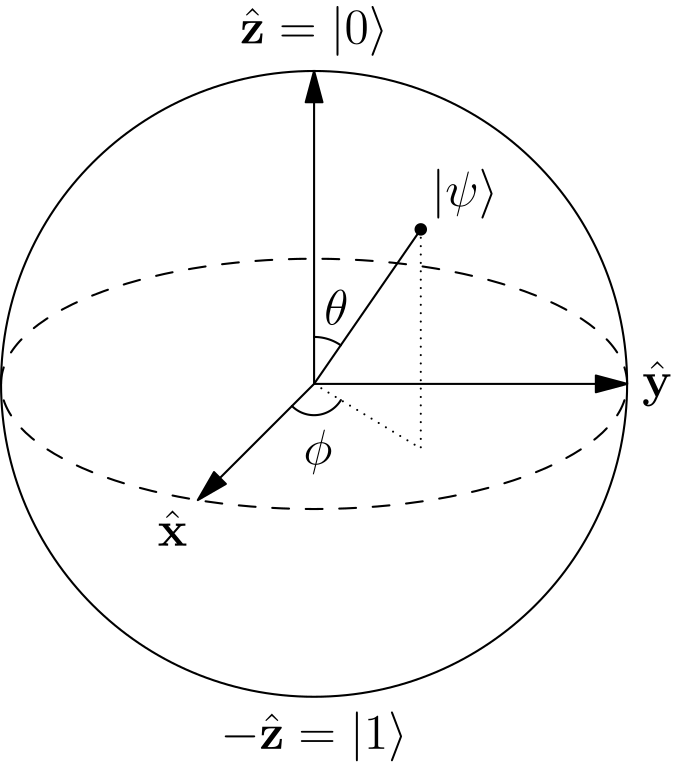
\includegraphics[width=0.4\linewidth]{Figures/677px-Bloch_Sphere.svg.png}
	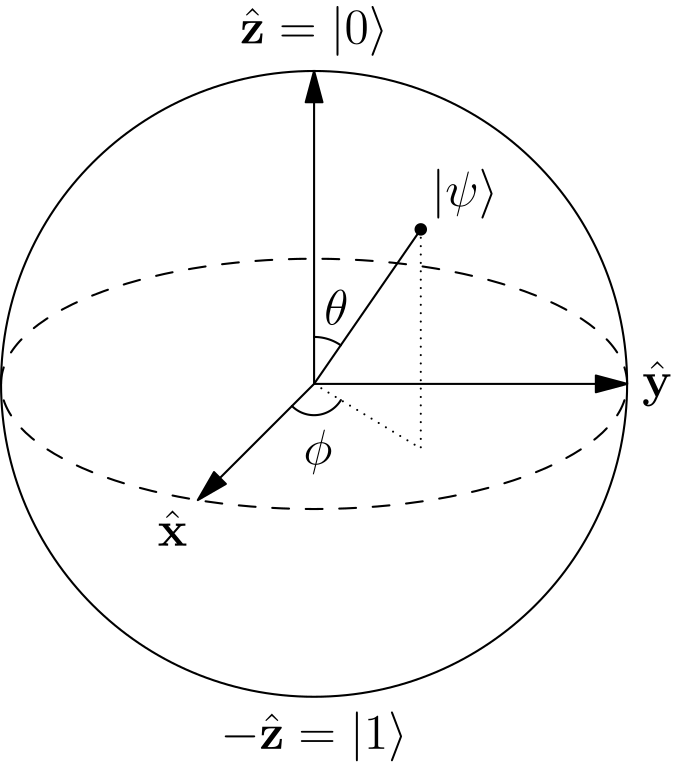
\includegraphics[width=0.4\linewidth]{Figures/677px-Bloch_Sphere.svg}
	\caption{Esfera de Bloch, on es representa un estat arbitrari $\ket{\psi}$ amb els vectors $\hat{\mathbf{x}}, \hat{\mathbf{y}}, \hat{\mathbf{z}}$ representat els eixos ortonormals de la esfera. }
	\label{fig:677px-blochsphere}
\end{figure}

%Glosser.ca, CC BY-SA 3.0 <https://creativecommons.org/licenses/by-sa/3.0>, via Wikimedia Commons
\subsection{Operacions per a només un qubit}
Una vegada es té la informació representada, estaria bé poder operar amb aquella informació, aquest es justament lo que fa que els ordinadors siguin ordinadors, poder operar amb la informació. En computació quàntica els qubits al poder ser representats amb vectors que tenen els seus coeficients són operats per les anomenades portes lògiques quàntiques, que són matrius. Per exemple, si es vol passar de tindre un qubit en l'estat $\ket{0}$ al estat $\ket{1}$, s'utilitza la porta lògica $X$ representada a continuació:
$$
X = \begin{bmatrix}
	0 & 1\\
	1 & 0\\
\end{bmatrix}
$$ 
Podem veure com fa l'acció al multiplicar la matriu per el vector: 
$$
\begin{bmatrix} 0 & 1\\ 1 & 0\\ \end{bmatrix} \begin{bmatrix}1 \\ 0 \end{bmatrix} = \begin{bmatrix}0 \\ 1 \end{bmatrix}
$$
Que en notació de Dirac s'expressaria com: 
$$
X\ket{0} = \ket{1}
$$
D'una manera més general: 
$$
\begin{bmatrix} 0 & 1\\ 1 & 0\\ \end{bmatrix} \begin{bmatrix}\alpha \\ \beta \end{bmatrix} =
\begin{bmatrix} 0\times\alpha & 1\times\beta \\
	1\times\alpha & 0\times\beta \\
\end{bmatrix}
 \begin{bmatrix} \beta \\ \alpha \end{bmatrix}

				1\times\alpha & 0\times\beta \\
\end{bmatrix}
 \begin{bmatrix} \beta \\ \alpha \end{bmatrix}
$$
Es pot veure que aquesta matriu lo que fa és donar la volta als coeficients d'un vector, per tant:
$$
X\ket{0} = \ket{1} \text{ i } X\ket{1} = \ket{0}
$$

Aquesta porta lògica forma part d'un grup important, les matrius de Pauli. Hi han 3 d'aquestes la X, la Y i la Z, usualment representades per $X$, $Y$, $Z$ o per $\sigma_x, \sigma_y, \sigma_z$. Aquestes matrius són les següents:
$$
	 X = \begin{bmatrix} 0 & 1\\ 1 & 0\\ \end{bmatrix} \; Y = \begin{bmatrix} 0 & i\\ -i & 0\\ \end{bmatrix} \; Z = \begin{bmatrix} 1 & 0\\ 0 & -1\\ \end{bmatrix} 
$$

Aquestes matrius són molt important en la mecànica quàntica\footnote{Al ser Hermitianes són observables, concretament ho són dels que corresponen al spin d'una partícula amb spin $\frac{1}{2}$ bàsicament estan relacionades amb els operadors del moment angular.} i són utilitzades àmpliament per descompondre i com a portes lògiques quàntiques.

A partir d'elles podem elaborar matrius que facin una rotació de qualsevol angle  en un del eixos de la representació geomètrica d'un qubit \ref{fig:677px-blochsphere}: 
\begin{align}
	& R_x(\theta) =  e^{-i\theta X/2} = \cos \frac{\theta}{2}I -i \sin \frac{\theta}{2}X = 
	\begin{bmatrix}
		\cos \frac{\theta}{2} & -i \sin \frac{\theta}{2} \\
		-i\sin \frac{\theta}{2} & \cos\frac{\theta}{2} \\
	\end{bmatrix} \label{eq:rx}\\
	& R_y(\theta) =  e^{-i\theta Y/2} = \cos \frac{\theta}{2}I -i \sin \frac{\theta}{2}Y = 
	\begin{bmatrix}
		\cos \frac{\theta}{2} & -\sin \frac{\theta}{2} \\
		\sin \frac{\theta}{2} & \cos\frac{\theta}{2} \\
	\end{bmatrix} \label{eq:ry}\\
	& R_y(\theta) =  e^{-i\theta Z/2} = \cos \frac{\theta}{2}I -i \sin \frac{\theta}{2}Z = 
	\begin{bmatrix}
		e^{-i\theta/2} & 0 \\
		0 & e^{i\theta/2} \\
	\end{bmatrix} \label{eq:rz}
\end{align}
Per exemple la matriu $R_y(\cdot)$ (Eq.\ref{eq:ry}) correspon a una rotació en el eix $\hat{\mathbf{y}}$ de la esfera de la figura \ref{fig:677px-blochsphere}. 
%The quantity of information that a qubit has is the information of all possible combination that the qubit has. One qubit has two possible combination $\ket{0}$ and $\ket{1}$, meanwhile two qubits have four possible combinations $\ket{00}, \ket{01}, \ket{10}, \ket{11}$, and four qubits have $2^4$ possible combinations, that is a total of $16$. And the information about each combination is a complex number, represent in the examples above has $\alpha_i$. The complex numbers are used to specify the quantum superposition that the system has. 

Aquestes operacions poden resultar en superposicions si es fan rotacions amb certs angles. Però hi ha una porta lògica especial per poder fer una rotació que resulta en una superposició \textit{no sé}. Es a dir una superposició que tingui les mateixes probabilitats de resultar en $\ket{0}$ o $\ket{1}$\footnote{Un 50\% cada una.}. Aquesta és la porta de Hadamard, denotada per $H$:
\begin{equation}
	H = \frac{1}{\sqrt{2}}\begin{bmatrix}
		1 & 1 \\ 1 & -1
	\end{bmatrix}
\end{equation}
Podem comprovar que és una superposició \textit{no sé} al aplicar-la al estat $\ket{0}$:

Aquesta porta lògica forma part d'un grup important, les matrius de Pauli. Hi han 3 d'aquestes la X, la Y i la Z, usualment representades per $X$, $Y$, $Z$ o per $\sigma_x, \sigma_y, \sigma_z$. Aquestes matrius són les següents:
\begin{enumerate}
	\item \textbf{Pauli-X:}
	$
	\begin{bmatrix} 0 & 1\\ 1 & 0\\ \end{bmatrix}
	$
	\item \textbf{Pauli-Y:}
	$
	\begin{bmatrix} i & 0\\ 0 & -i\\ \end{bmatrix}
	$
	\item \textbf{Pauli-Z:} 
	$
	\begin{bmatrix} 1 & 0\\ 0 & -1\\ \end{bmatrix}
	$
\end{enumerate}

Aquestes matrius corresponen a ractacioe s 

%The quantity of information that a qubit has is the information of all possible combination that the qubit has. One qubit has two possible combination $\ket{0}$ and $\ket{1}$, meanwhile two qubits have four possible combinations $\ket{00}, \ket{01}, \ket{10}, \ket{11}$, and four qubits have $2^4$ possible combinations, that is a total of $16$. And the information about each combination is a complex number, represent in the examples above has $\alpha_i$. The complex numbers are used to specify the quantum superposition that the system has. 

\subsection{Operacions per a múltiples qubits}

\section{Mesurament quàntic}
Tornant als fotons i la seva polarització, per prediu-re en quina base col·lapsa, necessitem utilitzar els mesuraments quàntics. Aquests mesuraments ens donen la probabilitat que té un fotó de col·lapsar en una certa base. 
On el vector $\ket{\text{\textrightarrow}}$ expressa la polarització d'un filtre i $\ket{\text{\textuparrow}}$ és el seu complement perpendicular, un fotó polaritzat té el estat següent \cite{QC_intro:photon}: 
$$
H\ket{0} = \frac{1}{\sqrt{2}}\begin{bmatrix}1 & 1 \\ 1 & -1 \end{bmatrix}\begin{bmatrix}1 \\ 0\end{bmatrix} = \begin{bmatrix} \frac{1}{\sqrt{2}} \\ \frac{1}{\sqrt{2}} \end{bmatrix}
$$
L'estat resultant és un estat especial que s'escriu com $\ket{+}$\footnote{Un altre estat similar és $\frac{\ket{0} - \ket{1}}{\sqrt{2}}$, quan la matriu $H$ s'aplica al estat $\ket{1}$.} La probabilitat de que un estat col·lapsi en una determinada base és el coeficient de la seva base elevat al quadrat. Com que l'estat és:
$$
\ket{+} = \begin{bmatrix} \frac{1}{\sqrt{2}} \\ \frac{1}{\sqrt{2}} \end{bmatrix} = \frac{\ket{0} + \ket{1}}{\sqrt{2}} =  \frac{1}{\sqrt{2}}\ket{0} +  \frac{1}{\sqrt{2}}\ket{1}
$$
Al elevar al quadrat qualsevol del coeficients es pot veure que dona $\frac{1}{2}$:
$$
\left(\frac{1}{\sqrt{2}}\right)^2 = \frac{1}{2}
$$
Llavors tenim que la probabilitat per obtindre ambos estats és la mateixa, es a dir que si mesurem l'estat $\ket{+}$ hi ha la mateixa probabilitat de que surti $\ket{0}$ o $\ket{1}$. La porta lògica de Hadamard és molt important ja que s'utilitza per crear distribucions uniformes, ja sigui en un qubit o en diversos \footnote{S'aplica aquesta operació a cada qubit del sistema.}. 

Altres operacions importants de només un qubit són les portes $S$ i $T$:
$$
S=\begin{bmatrix} 1 & 0 \\ 0 & 1 \end{bmatrix} \; \begin{bmatrix} 1 & 0 \\ 0 & e^{i\pi/4} \end{bmatrix}
$$
\subsection{Operacions per a múltiples qubits}
Lo realment interessant es quan s'apliquen portes a diversos qubits, perquè d'aquesta manera és pot arribar a tindre qubits entrellaçats. La porta més útil per entrellaçar qubits és la $\mathrm{CNOT}$ o \textit{Controlled NOT}:
La probabilitat de ser absorbit és $\alpha^2$, cal notar que $\alpha$ és el coeficient que correspon a la base $\ket{\text{\textrightarrow}}$, la base en la qual el filtre es orientat. En altres paraules, $\alpha^2$ indica la probabilitat del col·lapse de la polarització en l'estat $\ket{\text{\textrightarrow}}$. 

Els coeficients $\alpha$ i $\beta$ poden ser expressats com una funció del angle $\theta$\footnote{Per més informació sobre la polarització dels fotons, veure l'apèndix \ref{appendix:optics}.}
\begin{equation}
	\mathrm{CNOT} = 
	\begin{bmatrix}
		1 & 0 & 0 & 0 \\
		0 & 1 & 0 & 0 \\
		0 & 0 & 0 & 1 \\
		0 & 0 & 1 & 0 \\
	\end{bmatrix}
\end{equation}

És bàsicament una porta $X$\footnote{També anomenada porta $\mathrm{NOT}$ degut al paral·lelisme que es fa amb la porta lògica del ordinadors clàssics NOT \cite{wiki:NOT_gate} que simplement inverteix els bits d'1 a 0 (i viceversa), igual que $X$ que inverteix els qubits $\ket{1}$ a $\ket{0}$ i viceversa.} que està controlada per un altre qubit, si l'altre qubit és $\ket{1}$ s'aplica la porta $X$ al altre qubit. Però si l'altre qubit està en superposició, per exemple en $\ket{+}$, aquesta superposició es passa també al qubit controlat, i al mesurar el qubit, la probabilitat de que s'apliqui la porta $X$ és la probabilitat de mesurar l'estat $\ket{1}$. Es considera que aquests qubits estan entrellaçats, una mesura a un d'ells afecta a la mesura del altre. 

\subsubsection{Entrellaçament quàntic}
L'exemple més senzill d'un entrellaçament quàntic en la computació quàntica son els parells de Bell, que es creen al aplicar a dos qubits una porta $H$ al primer i després una porta $\mathrm{CNOT}$ als dos creant l'estat:
$$
\frac{\ket{00}+\ket{11}}{\sqrt{2}} = \frac{1}{\sqrt{2}}\ket{00} + \frac{1}{\sqrt{2}}\ket{11}
$$
Es pot veure que només hi han dos estats possibles $\ket{00}$ i $\ket{11}$ que tenen la mateixa probabilitat associada\footnote{Això es pot veure al elevar al quadrat els coeficients del dos, que donen $\frac{1}{2}$.}. S'afecten l'un al altre en el sentit que quan es mesura només un dels qubits i dona per exemple $\ket{1}$, al mesurar l'altre també dona $\ket{1}$, d'aquesta manera acabant amb l'estat $\ket{11}$. En altres paraules, la mesura d'una part del sistema determina el resultat d'una mesura en una altre part del sistema.

Matemàticament un sistema quàntic, e.i. un conjunt de qubits, està entrellaçant quan aquest sistema no es pot descriure amb un producte tensorial de les parts. Per exemple estat $\ket{00}$ es pot escriure com $\ket{0}\otimes\ket{0}$, mentre que l'estat $\frac{\ket{00} + \ket{11}}{\sqrt{2}}$, no. Per tant el primer no és sistema amb qubits entrellaçats i el segon si ho és.

A partir del entrellaçament i la superposició és com els ordinadors quàntics arribem a tenir avantatges en complexitat sobre els ordinadors clàssics, per més informació sobre els avantatges que presenten els algoritmes quàntics en certes tasques veure l'apèndix \ref{label}. \todo{appendix lol}

\section{Circuit quàntics}

%\section{Mesurament quàntic}
%Tornant als fotons i la seva polarització, per prediu-re en quina base col·lapsa, necessitem utilitzar els mesuraments quàntics. Aquests ens donen la probabilitat que té un fotó de col·lapsar en una certa base. 
%On el vector $\ket{\text{\textrightarrow}}$ expressa la polarització d'un filtre i $\ket{\text{\textuparrow}}$ és el seu complement perpendicular, un fotó polaritzat té el estat següent \cite{QC_intro:photon}: 
%$$
%\ket{\nearrow} = \alpha\ket{\text{\textrightarrow}} + \beta\ket{\text{\textuparrow}}
%$$
%La probabilitat de ser absorbit és $\alpha^2$, cal notar que $\alpha$ és el coeficient que correspon a la base $\ket{\text{\textrightarrow}}$, la base en la qual el filtre es orientat. En altres paraules, $\alpha^2$ indica la probabilitat del col·lapse de la polarització en l'estat $\ket{\text{\textrightarrow}}$. 

%Els coeficients $\alpha$ i $\beta$ poden ser expressats com una funció del angle $\theta$\footnote{Per més informació sobre la polarització dels fotons, veure l'apèndix \ref{appendix:optics}.}
%\begin{equation}
%	\ket{\nearrow} = \cos\theta\ket{\text{\textrightarrow}} + \sin\theta\ket{\text{\textuparrow}}
%	\label{eq:photon_state}
%\end{equation}
%I les probabilitats expectades es converteixen en $\cos^2\theta$ i $\sin^2\theta$, respectivament \cite{QC_intro:photon}. Ara podem mirar que els coeficients són la probabilitat, al veure el cas per $\theta = \pi/2$:
%\begin{align*}
%	p(\ket{\text{\textrightarrow}}) &= \cos^2\theta 
%	= \cos^2 \frac{\pi}{2}
%	= \left( \frac{1}{\sqrt{2}} \right) ^2 \\
%	&= 0.5 \\
%	p(\ket{\text{\textuparrow}}) &= \sin^2\theta 
%	= \sin^2 \frac{\pi}{2}
%	= \left( \frac{1}{\sqrt{2}} \right) ^2 \\
%	&= 0.5 \\	
%\end{align*} 

